\documentclass[dvipdfmx]{standalone}
\usepackage{tikz}
\usetikzlibrary{positioning}

\begin{document}
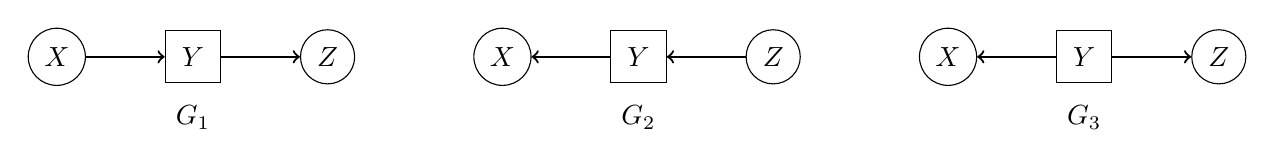
\begin{tikzpicture}[
  nodestyle/.style={
        draw,
        circle
  }
]

    \coordinate (G) at (0cm, 0cm);

    \node[nodestyle] (X_1) {$X$};
    \node[rectangle, draw, inner sep=6, right=1cm of X_1] (Y_1) {$Y$};
    \node[nodestyle, right=1cm of Y_1] (Z_1) {$Z$};
    \node[below = 0.5cm of Y_1.center]{$G_1$};

    \node[nodestyle, right=1.5cm of Z_1] (X_2) {$X$};
    \node[rectangle, draw, inner sep=6, right=1cm of X_2] (Y_2) {$Y$};
    \node[nodestyle, right=1cm of Y_2] (Z_2) {$Z$};
    \node[below = 0.5cm of Y_2.center]{$G_2$};

    \node[nodestyle, right=1.5cm of Z_2] (X_3) {$X$};
    \node[rectangle, draw, inner sep=6, right=1cm of X_3] (Y_3) {$Y$};
    \node[nodestyle, right=1cm of Y_3] (Z_3) {$Z$};
    \node[below = 0.5cm of Y_3.center]{$G_3$};

    \draw[thick, ->] (X_1) -- (Y_1);
    \draw[thick, ->] (Y_1) -- (Z_1);
    \draw[thick, ->] (Y_2) -- (X_2);
    \draw[thick, ->] (Z_2) -- (Y_2);
    \draw[thick, ->] (Y_3) -- (X_3);
    \draw[thick, ->] (Y_3) -- (Z_3);
\end{tikzpicture}
\end{document}
